% Options for packages loaded elsewhere
\PassOptionsToPackage{unicode}{hyperref}
\PassOptionsToPackage{hyphens}{url}
\PassOptionsToPackage{dvipsnames,svgnames,x11names}{xcolor}
%
\documentclass[
  ignorenonframetext,
]{beamer}
\usepackage{pgfpages}
\setbeamertemplate{caption}[numbered]
\setbeamertemplate{caption label separator}{: }
\setbeamercolor{caption name}{fg=normal text.fg}
\beamertemplatenavigationsymbolsempty
% Prevent slide breaks in the middle of a paragraph
\widowpenalties 1 10000
\raggedbottom

\usepackage{amsmath,amssymb}
\usepackage{iftex}
\ifPDFTeX
  \usepackage[T1]{fontenc}
  \usepackage[utf8]{inputenc}
  \usepackage{textcomp} % provide euro and other symbols
\else % if luatex or xetex
  \usepackage{unicode-math}
  \defaultfontfeatures{Scale=MatchLowercase}
  \defaultfontfeatures[\rmfamily]{Ligatures=TeX,Scale=1}
\fi
\usepackage{lmodern}
\usetheme[]{AnnArbor}
\usecolortheme{dolphin}
\usefonttheme{structurebold}
\ifPDFTeX\else  
    % xetex/luatex font selection
\fi
% Use upquote if available, for straight quotes in verbatim environments
\IfFileExists{upquote.sty}{\usepackage{upquote}}{}
\IfFileExists{microtype.sty}{% use microtype if available
  \usepackage[]{microtype}
  \UseMicrotypeSet[protrusion]{basicmath} % disable protrusion for tt fonts
}{}
\makeatletter
\@ifundefined{KOMAClassName}{% if non-KOMA class
  \IfFileExists{parskip.sty}{%
    \usepackage{parskip}
  }{% else
    \setlength{\parindent}{0pt}
    \setlength{\parskip}{6pt plus 2pt minus 1pt}}
}{% if KOMA class
  \KOMAoptions{parskip=half}}
\makeatother
\usepackage{xcolor}
\newif\ifbibliography
\setlength{\emergencystretch}{3em} % prevent overfull lines
\setcounter{secnumdepth}{-\maxdimen} % remove section numbering

\usepackage{color}
\usepackage{fancyvrb}
\newcommand{\VerbBar}{|}
\newcommand{\VERB}{\Verb[commandchars=\\\{\}]}
\DefineVerbatimEnvironment{Highlighting}{Verbatim}{commandchars=\\\{\}}
% Add ',fontsize=\small' for more characters per line
\usepackage{framed}
\definecolor{shadecolor}{RGB}{241,243,245}
\newenvironment{Shaded}{\begin{snugshade}}{\end{snugshade}}
\newcommand{\AlertTok}[1]{\textcolor[rgb]{0.68,0.00,0.00}{#1}}
\newcommand{\AnnotationTok}[1]{\textcolor[rgb]{0.37,0.37,0.37}{#1}}
\newcommand{\AttributeTok}[1]{\textcolor[rgb]{0.40,0.45,0.13}{#1}}
\newcommand{\BaseNTok}[1]{\textcolor[rgb]{0.68,0.00,0.00}{#1}}
\newcommand{\BuiltInTok}[1]{\textcolor[rgb]{0.00,0.23,0.31}{#1}}
\newcommand{\CharTok}[1]{\textcolor[rgb]{0.13,0.47,0.30}{#1}}
\newcommand{\CommentTok}[1]{\textcolor[rgb]{0.37,0.37,0.37}{#1}}
\newcommand{\CommentVarTok}[1]{\textcolor[rgb]{0.37,0.37,0.37}{\textit{#1}}}
\newcommand{\ConstantTok}[1]{\textcolor[rgb]{0.56,0.35,0.01}{#1}}
\newcommand{\ControlFlowTok}[1]{\textcolor[rgb]{0.00,0.23,0.31}{\textbf{#1}}}
\newcommand{\DataTypeTok}[1]{\textcolor[rgb]{0.68,0.00,0.00}{#1}}
\newcommand{\DecValTok}[1]{\textcolor[rgb]{0.68,0.00,0.00}{#1}}
\newcommand{\DocumentationTok}[1]{\textcolor[rgb]{0.37,0.37,0.37}{\textit{#1}}}
\newcommand{\ErrorTok}[1]{\textcolor[rgb]{0.68,0.00,0.00}{#1}}
\newcommand{\ExtensionTok}[1]{\textcolor[rgb]{0.00,0.23,0.31}{#1}}
\newcommand{\FloatTok}[1]{\textcolor[rgb]{0.68,0.00,0.00}{#1}}
\newcommand{\FunctionTok}[1]{\textcolor[rgb]{0.28,0.35,0.67}{#1}}
\newcommand{\ImportTok}[1]{\textcolor[rgb]{0.00,0.46,0.62}{#1}}
\newcommand{\InformationTok}[1]{\textcolor[rgb]{0.37,0.37,0.37}{#1}}
\newcommand{\KeywordTok}[1]{\textcolor[rgb]{0.00,0.23,0.31}{\textbf{#1}}}
\newcommand{\NormalTok}[1]{\textcolor[rgb]{0.00,0.23,0.31}{#1}}
\newcommand{\OperatorTok}[1]{\textcolor[rgb]{0.37,0.37,0.37}{#1}}
\newcommand{\OtherTok}[1]{\textcolor[rgb]{0.00,0.23,0.31}{#1}}
\newcommand{\PreprocessorTok}[1]{\textcolor[rgb]{0.68,0.00,0.00}{#1}}
\newcommand{\RegionMarkerTok}[1]{\textcolor[rgb]{0.00,0.23,0.31}{#1}}
\newcommand{\SpecialCharTok}[1]{\textcolor[rgb]{0.37,0.37,0.37}{#1}}
\newcommand{\SpecialStringTok}[1]{\textcolor[rgb]{0.13,0.47,0.30}{#1}}
\newcommand{\StringTok}[1]{\textcolor[rgb]{0.13,0.47,0.30}{#1}}
\newcommand{\VariableTok}[1]{\textcolor[rgb]{0.07,0.07,0.07}{#1}}
\newcommand{\VerbatimStringTok}[1]{\textcolor[rgb]{0.13,0.47,0.30}{#1}}
\newcommand{\WarningTok}[1]{\textcolor[rgb]{0.37,0.37,0.37}{\textit{#1}}}

\providecommand{\tightlist}{%
  \setlength{\itemsep}{0pt}\setlength{\parskip}{0pt}}\usepackage{longtable,booktabs,array}
\usepackage{calc} % for calculating minipage widths
\usepackage{caption}
% Make caption package work with longtable
\makeatletter
\def\fnum@table{\tablename~\thetable}
\makeatother
\usepackage{graphicx}
\makeatletter
\def\maxwidth{\ifdim\Gin@nat@width>\linewidth\linewidth\else\Gin@nat@width\fi}
\def\maxheight{\ifdim\Gin@nat@height>\textheight\textheight\else\Gin@nat@height\fi}
\makeatother
% Scale images if necessary, so that they will not overflow the page
% margins by default, and it is still possible to overwrite the defaults
% using explicit options in \includegraphics[width, height, ...]{}
\setkeys{Gin}{width=\maxwidth,height=\maxheight,keepaspectratio}
% Set default figure placement to htbp
\makeatletter
\def\fps@figure{htbp}
\makeatother
% definitions for citeproc citations
\NewDocumentCommand\citeproctext{}{}
\NewDocumentCommand\citeproc{mm}{%
  \begingroup\def\citeproctext{#2}\cite{#1}\endgroup}
\makeatletter
 % allow citations to break across lines
 \let\@cite@ofmt\@firstofone
 % avoid brackets around text for \cite:
 \def\@biblabel#1{}
 \def\@cite#1#2{{#1\if@tempswa , #2\fi}}
\makeatother
\newlength{\cslhangindent}
\setlength{\cslhangindent}{1.5em}
\newlength{\csllabelwidth}
\setlength{\csllabelwidth}{3em}
\newenvironment{CSLReferences}[2] % #1 hanging-indent, #2 entry-spacing
 {\begin{list}{}{%
  \setlength{\itemindent}{0pt}
  \setlength{\leftmargin}{0pt}
  \setlength{\parsep}{0pt}
  % turn on hanging indent if param 1 is 1
  \ifodd #1
   \setlength{\leftmargin}{\cslhangindent}
   \setlength{\itemindent}{-1\cslhangindent}
  \fi
  % set entry spacing
  \setlength{\itemsep}{#2\baselineskip}}}
 {\end{list}}
\usepackage{calc}
\newcommand{\CSLBlock}[1]{\hfill\break\parbox[t]{\linewidth}{\strut\ignorespaces#1\strut}}
\newcommand{\CSLLeftMargin}[1]{\parbox[t]{\csllabelwidth}{\strut#1\strut}}
\newcommand{\CSLRightInline}[1]{\parbox[t]{\linewidth - \csllabelwidth}{\strut#1\strut}}
\newcommand{\CSLIndent}[1]{\hspace{\cslhangindent}#1}


% logo
\titlegraphic{
\includegraphics[width=4cm]{../000_logos/logo-blue-vertical}}
\logo{\ifnum\thepage>1
\includegraphics[width=0.5cm]{../000_logos/logo-blue-vertical}\fi}

% UMNG: Manual de image institucional

% Colors

% Umng
\definecolor{yellow}{HTML}{fdc600}
\definecolor{red}{HTML}{ee2a24}

% Estudios a Distancia
\definecolor{blue1}{HTML}{12245b}
\definecolor{blue2}{HTML}{767ca6}
\definecolor{blue3}{HTML}{cad2ec}

% Modify items
\setbeamercolor{palette primary}{bg=blue3}
\setbeamercolor{palette tertiary}{bg=blue1}
\setbeamercolor{frametitle}{bg=yellow}

% Hyperlinks
\hypersetup{
  linkcolor=red,
  citecolor=red
}

\makeatletter
\@ifpackageloaded{caption}{}{\usepackage{caption}}
\AtBeginDocument{%
\ifdefined\contentsname
  \renewcommand*\contentsname{Table of contents}
\else
  \newcommand\contentsname{Table of contents}
\fi
\ifdefined\listfigurename
  \renewcommand*\listfigurename{List of Figures}
\else
  \newcommand\listfigurename{List of Figures}
\fi
\ifdefined\listtablename
  \renewcommand*\listtablename{List of Tables}
\else
  \newcommand\listtablename{List of Tables}
\fi
\ifdefined\figurename
  \renewcommand*\figurename{Figure}
\else
  \newcommand\figurename{Figure}
\fi
\ifdefined\tablename
  \renewcommand*\tablename{Table}
\else
  \newcommand\tablename{Table}
\fi
}
\@ifpackageloaded{float}{}{\usepackage{float}}
\floatstyle{ruled}
\@ifundefined{c@chapter}{\newfloat{codelisting}{h}{lop}}{\newfloat{codelisting}{h}{lop}[chapter]}
\floatname{codelisting}{Listing}
\newcommand*\listoflistings{\listof{codelisting}{List of Listings}}
\makeatother
\makeatletter
\makeatother
\makeatletter
\@ifpackageloaded{caption}{}{\usepackage{caption}}
\@ifpackageloaded{subcaption}{}{\usepackage{subcaption}}
\makeatother

\ifLuaTeX
\usepackage[bidi=basic]{babel}
\else
\usepackage[bidi=default]{babel}
\fi
\babelprovide[main,import]{english}
% get rid of language-specific shorthands (see #6817):
\let\LanguageShortHands\languageshorthands
\def\languageshorthands#1{}
\ifLuaTeX
  \usepackage{selnolig}  % disable illegal ligatures
\fi
\usepackage{bookmark}

\IfFileExists{xurl.sty}{\usepackage{xurl}}{} % add URL line breaks if available
\urlstyle{same} % disable monospaced font for URLs
\hypersetup{
  pdftitle={Comparing Groups: Tables and Visualizations},
  pdfauthor={Luis Francisco Gómez López},
  pdflang={en},
  colorlinks=true,
  linkcolor={Maroon},
  filecolor={Maroon},
  citecolor={Blue},
  urlcolor={Blue},
  pdfcreator={LaTeX via pandoc}}


\title{Comparing Groups: Tables and Visualizations}
\author{Luis Francisco Gómez López}
\date{2024-08-01}
\institute{FAEDIS}

\begin{document}
\frame{\titlepage}

\renewcommand*\contentsname{Table of contents}
\begin{frame}[allowframebreaks]
  \frametitle{Table of contents}
  \tableofcontents[hideallsubsections]
\end{frame}

\section{Please Read Me}\label{please-read-me}

\begin{frame}{}
\phantomsection\label{section}
\begin{itemize}
\tightlist
\item
  This presentation is based on (\citeproc{ref-chapman_r_2019}{Chapman
  and Feit 2019, chap. 5})
\end{itemize}
\end{frame}

\section{Purpose}\label{purpose}

\begin{frame}{}
\phantomsection\label{section-1}
\begin{itemize}
\tightlist
\item
  Use descriptive summaries by groups and visualize them to investigate
  differences between groups
\end{itemize}
\end{frame}

\section{Consumer segmentation
survey}\label{consumer-segmentation-survey}

\begin{frame}{}
\phantomsection\label{section-2}
\begin{itemize}
\tightlist
\item
  \textbf{age}: age of the consumer in years
\item
  \textbf{gender}: if the consumer is male of female
\item
  \textbf{income}: yearly disposable income of the consumer
\item
  \textbf{kids}: number of children of the consumer
\item
  \textbf{ownHome}: if the consumer owns a home
\item
  \textbf{subscribe}: if the consumer is subscribed or not
\item
  \textbf{Segment}: market segment assigned by a clustering algorithm
  (\citeproc{ref-chapman_r_2019}{Chapman and Feit 2019, chap. 11}),
  expert assignment or a segmentation typing tool
\end{itemize}
\end{frame}

\begin{frame}{}
\phantomsection\label{section-3}
\begin{itemize}
\item
  \textbf{Segment}:

  \begin{itemize}
  \tightlist
  \item
    \textbf{Moving up}: consumers experiencing upward mobility in terms
    of their socioeconomic status
  \item
    \textbf{Suburb mix}: consumers living in suburban areas
  \item
    \textbf{Travelers}: consumers who prioritize experiences and
    adventures
  \item
    \textbf{Urban Hip}: consumers interested in urban culture, artistic
    expression, and modern trends
  \end{itemize}
\end{itemize}
\end{frame}

\begin{frame}[fragile]{}
\phantomsection\label{section-4}
\begin{itemize}
\tightlist
\item
  \textbf{Import data}
\end{itemize}

\tiny

\begin{Shaded}
\begin{Highlighting}[]
\NormalTok{segmentation }\OtherTok{\textless{}{-}} \FunctionTok{read\_csv}\NormalTok{(}\AttributeTok{file =} \StringTok{"http://goo.gl/qw303p"}\NormalTok{)}
\NormalTok{segmentation }\SpecialCharTok{|\textgreater{}} \FunctionTok{head}\NormalTok{(}\AttributeTok{n =} \DecValTok{5}\NormalTok{)}
\end{Highlighting}
\end{Shaded}

\begin{verbatim}
# A tibble: 5 x 7
    age gender income  kids ownHome subscribe Segment   
  <dbl> <chr>   <dbl> <dbl> <chr>   <chr>     <chr>     
1  47.3 Male   49483.     2 ownNo   subNo     Suburb mix
2  31.4 Male   35546.     1 ownYes  subNo     Suburb mix
3  43.2 Male   44169.     0 ownYes  subNo     Suburb mix
4  37.3 Female 81042.     1 ownNo   subNo     Suburb mix
5  41.0 Female 79353.     3 ownYes  subNo     Suburb mix
\end{verbatim}
\end{frame}

\begin{frame}[fragile]{}
\phantomsection\label{section-5}
\begin{itemize}
\tightlist
\item
  \textbf{Transform data}
\end{itemize}

\tiny

\begin{Shaded}
\begin{Highlighting}[]
\NormalTok{segmentation }\OtherTok{\textless{}{-}}\NormalTok{ segmentation }\SpecialCharTok{|\textgreater{}}
  \FunctionTok{mutate}\NormalTok{(}\AttributeTok{gender =} \FunctionTok{factor}\NormalTok{(gender, }\AttributeTok{ordered =} \ConstantTok{FALSE}\NormalTok{),}
         \AttributeTok{kids =} \FunctionTok{as.integer}\NormalTok{(kids),}
         \AttributeTok{ownHome =} \FunctionTok{factor}\NormalTok{(ownHome, }\AttributeTok{ordered =} \ConstantTok{FALSE}\NormalTok{),}
         \AttributeTok{subscribe =} \FunctionTok{factor}\NormalTok{(subscribe, }\AttributeTok{ordered =} \ConstantTok{FALSE}\NormalTok{),}
         \AttributeTok{Segment =} \FunctionTok{factor}\NormalTok{(Segment, }\AttributeTok{ordered =} \ConstantTok{FALSE}\NormalTok{))}

\NormalTok{segmentation }\SpecialCharTok{|\textgreater{}} \FunctionTok{head}\NormalTok{(}\AttributeTok{n =} \DecValTok{5}\NormalTok{)}
\end{Highlighting}
\end{Shaded}

\begin{verbatim}
# A tibble: 5 x 7
    age gender income  kids ownHome subscribe Segment   
  <dbl> <fct>   <dbl> <int> <fct>   <fct>     <fct>     
1  47.3 Male   49483.     2 ownNo   subNo     Suburb mix
2  31.4 Male   35546.     1 ownYes  subNo     Suburb mix
3  43.2 Male   44169.     0 ownYes  subNo     Suburb mix
4  37.3 Female 81042.     1 ownNo   subNo     Suburb mix
5  41.0 Female 79353.     3 ownYes  subNo     Suburb mix
\end{verbatim}
\end{frame}

\begin{frame}[fragile]{}
\phantomsection\label{section-6}
\begin{itemize}
\item
  \textbf{Basic Formula Syntax}

  \begin{itemize}
  \item
    \(\sim\) and \(+\): operators
  \item
    \(y\): response variable
  \item
    \(x, z\): explanatory variables
  \item
    \(y \sim x + z\): a formula which means that \(y\) depends on \(x\)
    and \(z\)

    \begin{itemize}
    \tightlist
    \item
      \(+\) is used to indicate the addition of predictor variables to
      the right of the formula
    \item
      Be careful not to confuse the arithmetic operator \(+\) with \(+\)
      within a formula
    \end{itemize}
  \end{itemize}
\end{itemize}

\tiny

\begin{Shaded}
\begin{Highlighting}[]
\NormalTok{?}\StringTok{\textasciigrave{}}\AttributeTok{+}\StringTok{\textasciigrave{}} \CommentTok{\# Arithmetic Operators}
\NormalTok{?formula }\CommentTok{\# operators in a formula}
\end{Highlighting}
\end{Shaded}
\end{frame}

\begin{frame}[fragile]{}
\phantomsection\label{section-7}
\begin{itemize}
\item
  \textbf{Descriptives for n-Way Groups: the base R way}

  \begin{itemize}
  \tightlist
  \item
    Split data into \(n\) subsets and compute summary statistics
  \end{itemize}
\end{itemize}

\tiny

\begin{Shaded}
\begin{Highlighting}[]
\FunctionTok{aggregate}\NormalTok{(}\AttributeTok{x =}\NormalTok{ income }\SpecialCharTok{\textasciitilde{}}\NormalTok{ Segment }\SpecialCharTok{+}\NormalTok{ ownHome, }
          \AttributeTok{data =}\NormalTok{ segmentation, }\AttributeTok{FUN =}\NormalTok{ mean)}
\end{Highlighting}
\end{Shaded}

\begin{verbatim}
     Segment ownHome   income
1  Moving up   ownNo 54497.68
2 Suburb mix   ownNo 54932.83
3  Travelers   ownNo 63188.42
4  Urban hip   ownNo 21337.59
5  Moving up  ownYes 50216.37
6 Suburb mix  ownYes 55143.21
7  Travelers  ownYes 61889.12
8  Urban hip  ownYes 23059.27
\end{verbatim}
\end{frame}

\begin{frame}[fragile]{}
\phantomsection\label{section-8}
\begin{itemize}
\item
  \textbf{Descriptives for n-Way Groups: the base R way}

  \begin{itemize}
  \tightlist
  \item
    Split data into \(n\) subsets and compute summary statistics
  \end{itemize}
\end{itemize}

\tiny

\begin{Shaded}
\begin{Highlighting}[]
\FunctionTok{aggregate}\NormalTok{(}\AttributeTok{x =}\NormalTok{ kids }\SpecialCharTok{\textasciitilde{}}\NormalTok{ Segment }\SpecialCharTok{+}\NormalTok{ ownHome, }
          \AttributeTok{data =}\NormalTok{ segmentation, }\AttributeTok{FUN =}\NormalTok{ sum)}
\end{Highlighting}
\end{Shaded}

\begin{verbatim}
     Segment ownHome kids
1  Moving up   ownNo   82
2 Suburb mix   ownNo   90
3  Travelers   ownNo    0
4  Urban hip   ownNo   43
5  Moving up  ownYes   52
6 Suburb mix  ownYes  102
7  Travelers  ownYes    0
8  Urban hip  ownYes   12
\end{verbatim}
\end{frame}

\begin{frame}[fragile]{}
\phantomsection\label{section-9}
\begin{itemize}
\item
  \textbf{Descriptives for n-Way Groups: the tidyverse way}

  \begin{itemize}
  \tightlist
  \item
    Split data into \(n\) subsets and compute summary statistics
  \end{itemize}
\end{itemize}

\tiny

\begin{Shaded}
\begin{Highlighting}[]
\NormalTok{segmentation }\SpecialCharTok{|\textgreater{}} 
  \FunctionTok{group\_by}\NormalTok{(Segment, ownHome) }\SpecialCharTok{|\textgreater{}}
  \FunctionTok{summarise}\NormalTok{(}\AttributeTok{mean\_income =} \FunctionTok{mean}\NormalTok{(income))}
\end{Highlighting}
\end{Shaded}

\begin{verbatim}
# A tibble: 8 x 3
# Groups:   Segment [4]
  Segment    ownHome mean_income
  <fct>      <fct>         <dbl>
1 Moving up  ownNo        54498.
2 Moving up  ownYes       50216.
3 Suburb mix ownNo        54933.
4 Suburb mix ownYes       55143.
5 Travelers  ownNo        63188.
6 Travelers  ownYes       61889.
7 Urban hip  ownNo        21338.
8 Urban hip  ownYes       23059.
\end{verbatim}
\end{frame}

\begin{frame}[fragile]{}
\phantomsection\label{section-10}
\begin{itemize}
\item
  \textbf{Descriptives for n-Way Groups: the tidyverse way}

  \begin{itemize}
  \tightlist
  \item
    Split data into \(n\) subsets and compute summary statistics
  \end{itemize}
\end{itemize}

\tiny

\begin{Shaded}
\begin{Highlighting}[]
\NormalTok{segmentation }\SpecialCharTok{|\textgreater{}} 
  \FunctionTok{group\_by}\NormalTok{(Segment, ownHome) }\SpecialCharTok{|\textgreater{}}
  \FunctionTok{summarise}\NormalTok{(}\AttributeTok{sum\_kids =} \FunctionTok{sum}\NormalTok{(kids))}
\end{Highlighting}
\end{Shaded}

\begin{verbatim}
# A tibble: 8 x 3
# Groups:   Segment [4]
  Segment    ownHome sum_kids
  <fct>      <fct>      <int>
1 Moving up  ownNo         82
2 Moving up  ownYes        52
3 Suburb mix ownNo         90
4 Suburb mix ownYes       102
5 Travelers  ownNo          0
6 Travelers  ownYes         0
7 Urban hip  ownNo         43
8 Urban hip  ownYes        12
\end{verbatim}
\end{frame}

\begin{frame}[fragile]{}
\phantomsection\label{section-11}
\begin{itemize}
\item
  \textbf{Basic Formula Syntax}

  \begin{itemize}
  \item
    \(\sim\), \(+\) and \(|\): operators
  \item
    \(y\): response variable
  \item
    \(x\): explanatory variable
  \item
    \(z\): grouping variable
  \item
    \(y \sim x | z\): \(y\) depends on \(x\) based on different groups
    defined by \(z\)

    \begin{itemize}
    \tightlist
    \item
      \(|\) is used to separate the grouping variable from the
      explanatory variable
    \item
      Be careful not to confuse the logical operator \(|\) with \(|\)
      within a formula
    \end{itemize}
  \end{itemize}
\end{itemize}

\tiny

\begin{Shaded}
\begin{Highlighting}[]
\NormalTok{?}\StringTok{\textasciigrave{}}\AttributeTok{|}\StringTok{\textasciigrave{}} \CommentTok{\# Logical Operators}
\NormalTok{?lattice}\SpecialCharTok{::}\NormalTok{xyplot }\CommentTok{\# operators in a formula (you need first to install the package lattice)}
\end{Highlighting}
\end{Shaded}
\end{frame}

\begin{frame}[fragile]{}
\phantomsection\label{section-12}
\begin{itemize}
\tightlist
\item
  \textbf{Visualization by group as frequencies: the lattice way}
\end{itemize}

\tiny

\begin{Shaded}
\begin{Highlighting}[]
\FunctionTok{library}\NormalTok{(lattice)}
\FunctionTok{histogram}\NormalTok{(}\SpecialCharTok{\textasciitilde{}}\NormalTok{ subscribe }\SpecialCharTok{|}\NormalTok{ Segment }\SpecialCharTok{+}\NormalTok{ ownHome, }\AttributeTok{data =}\NormalTok{ segmentation)}
\end{Highlighting}
\end{Shaded}

\begin{center}
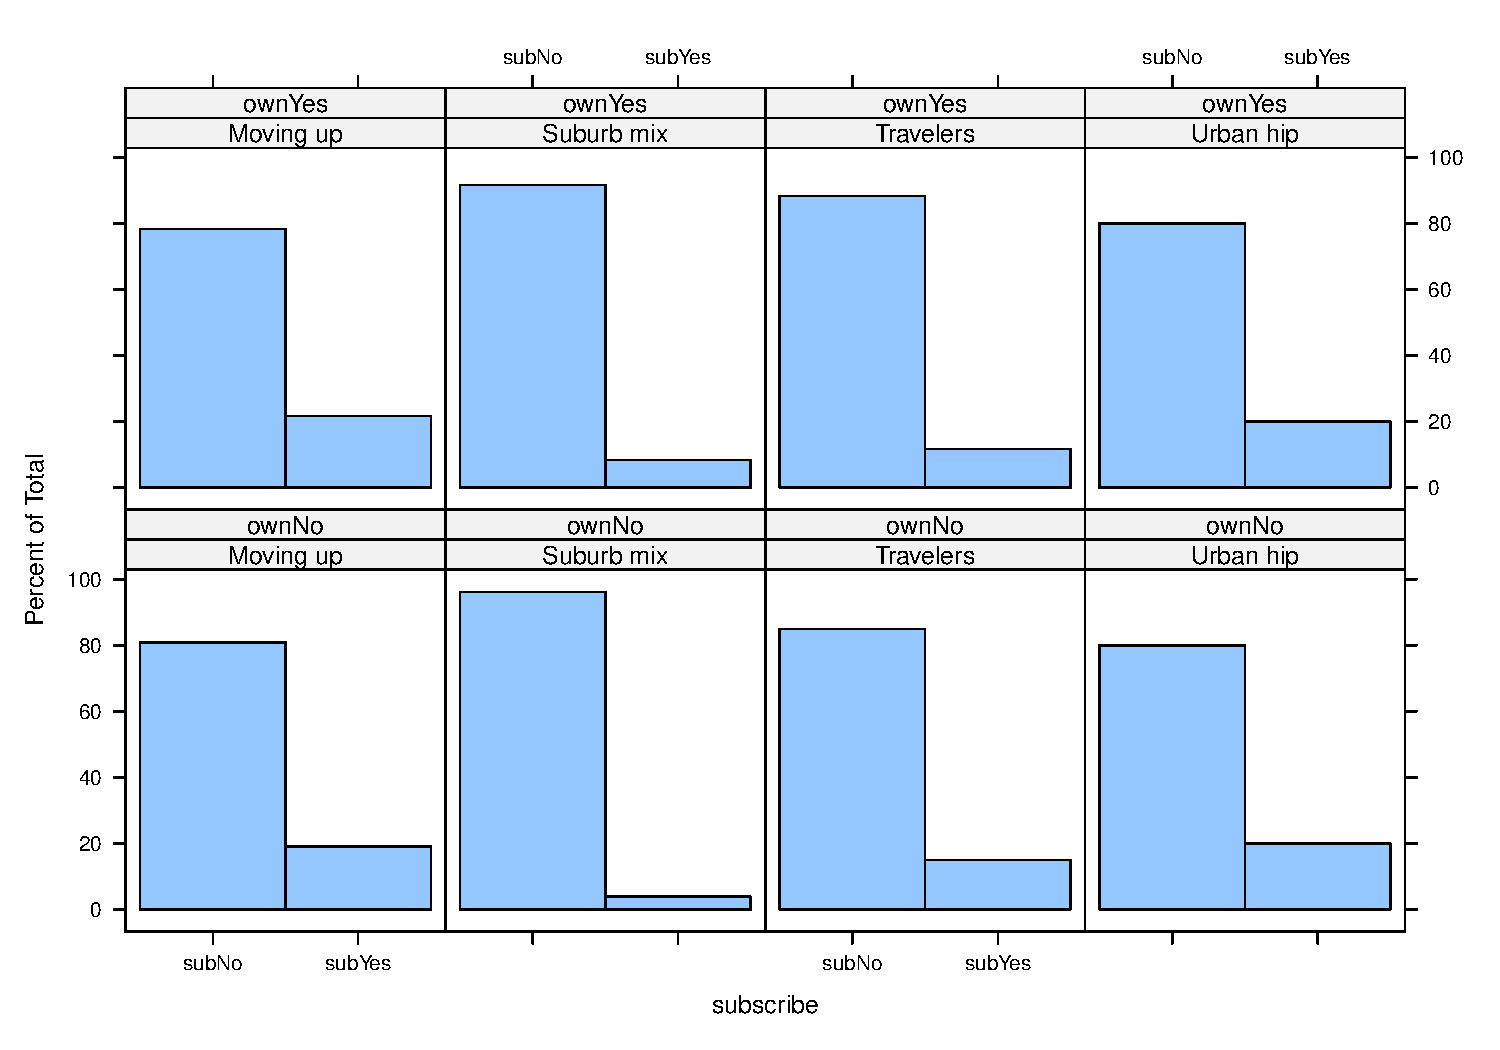
\includegraphics[width=0.5\textwidth,height=\textheight]{005_comparing_groups_tables_and_visualizations_files/figure-beamer/unnamed-chunk-10-1.pdf}
\end{center}
\end{frame}

\begin{frame}[fragile]{}
\phantomsection\label{section-13}
\begin{itemize}
\tightlist
\item
  \textbf{Visualization by group as frequencies: the tidyverse way}
\end{itemize}

\tiny

\begin{Shaded}
\begin{Highlighting}[]
\CommentTok{\# Prepare data}
\NormalTok{subscriber\_by\_segment\_home\_ownership }\OtherTok{\textless{}{-}}\NormalTok{ segmentation }\SpecialCharTok{|\textgreater{}}
  \FunctionTok{count}\NormalTok{(subscribe, Segment, ownHome) }\SpecialCharTok{|\textgreater{}}
  \FunctionTok{group\_by}\NormalTok{(Segment, ownHome) }\SpecialCharTok{|\textgreater{}}
  \FunctionTok{mutate}\NormalTok{(}\AttributeTok{n\_pct =}\NormalTok{ (n }\SpecialCharTok{/} \FunctionTok{sum}\NormalTok{(n)) }\SpecialCharTok{*} \DecValTok{100}\NormalTok{) }\SpecialCharTok{|\textgreater{}}
  \FunctionTok{ungroup}\NormalTok{()}
\NormalTok{subscriber\_by\_segment\_home\_ownership}
\end{Highlighting}
\end{Shaded}

\begin{verbatim}
# A tibble: 16 x 5
   subscribe Segment    ownHome     n n_pct
   <fct>     <fct>      <fct>   <int> <dbl>
 1 subNo     Moving up  ownNo      38 80.9 
 2 subNo     Moving up  ownYes     18 78.3 
 3 subNo     Suburb mix ownNo      50 96.2 
 4 subNo     Suburb mix ownYes     44 91.7 
 5 subNo     Travelers  ownNo      17 85   
 6 subNo     Travelers  ownYes     53 88.3 
 7 subNo     Urban hip  ownNo      32 80   
 8 subNo     Urban hip  ownYes      8 80   
 9 subYes    Moving up  ownNo       9 19.1 
10 subYes    Moving up  ownYes      5 21.7 
11 subYes    Suburb mix ownNo       2  3.85
12 subYes    Suburb mix ownYes      4  8.33
13 subYes    Travelers  ownNo       3 15   
14 subYes    Travelers  ownYes      7 11.7 
15 subYes    Urban hip  ownNo       8 20   
16 subYes    Urban hip  ownYes      2 20   
\end{verbatim}
\end{frame}

\begin{frame}[fragile]{}
\phantomsection\label{section-14}
\begin{itemize}
\tightlist
\item
  \textbf{Visualization by group as frequencies: the tidyverse way}
\end{itemize}

\tiny

\begin{Shaded}
\begin{Highlighting}[]
\NormalTok{subscriber\_by\_segment\_home\_ownership }\SpecialCharTok{|\textgreater{}}
  \FunctionTok{ggplot}\NormalTok{() }\SpecialCharTok{+} 
  \FunctionTok{geom\_col}\NormalTok{(}\FunctionTok{aes}\NormalTok{(}\AttributeTok{x =}\NormalTok{ subscribe, }\AttributeTok{y=}\NormalTok{n\_pct)) }\SpecialCharTok{+} 
  \FunctionTok{facet\_wrap}\NormalTok{(}\AttributeTok{facets =} \FunctionTok{vars}\NormalTok{(Segment,ownHome), }
             \AttributeTok{nrow =} \DecValTok{2}\NormalTok{, }\AttributeTok{ncol =} \DecValTok{4}\NormalTok{)}
\end{Highlighting}
\end{Shaded}

\begin{center}
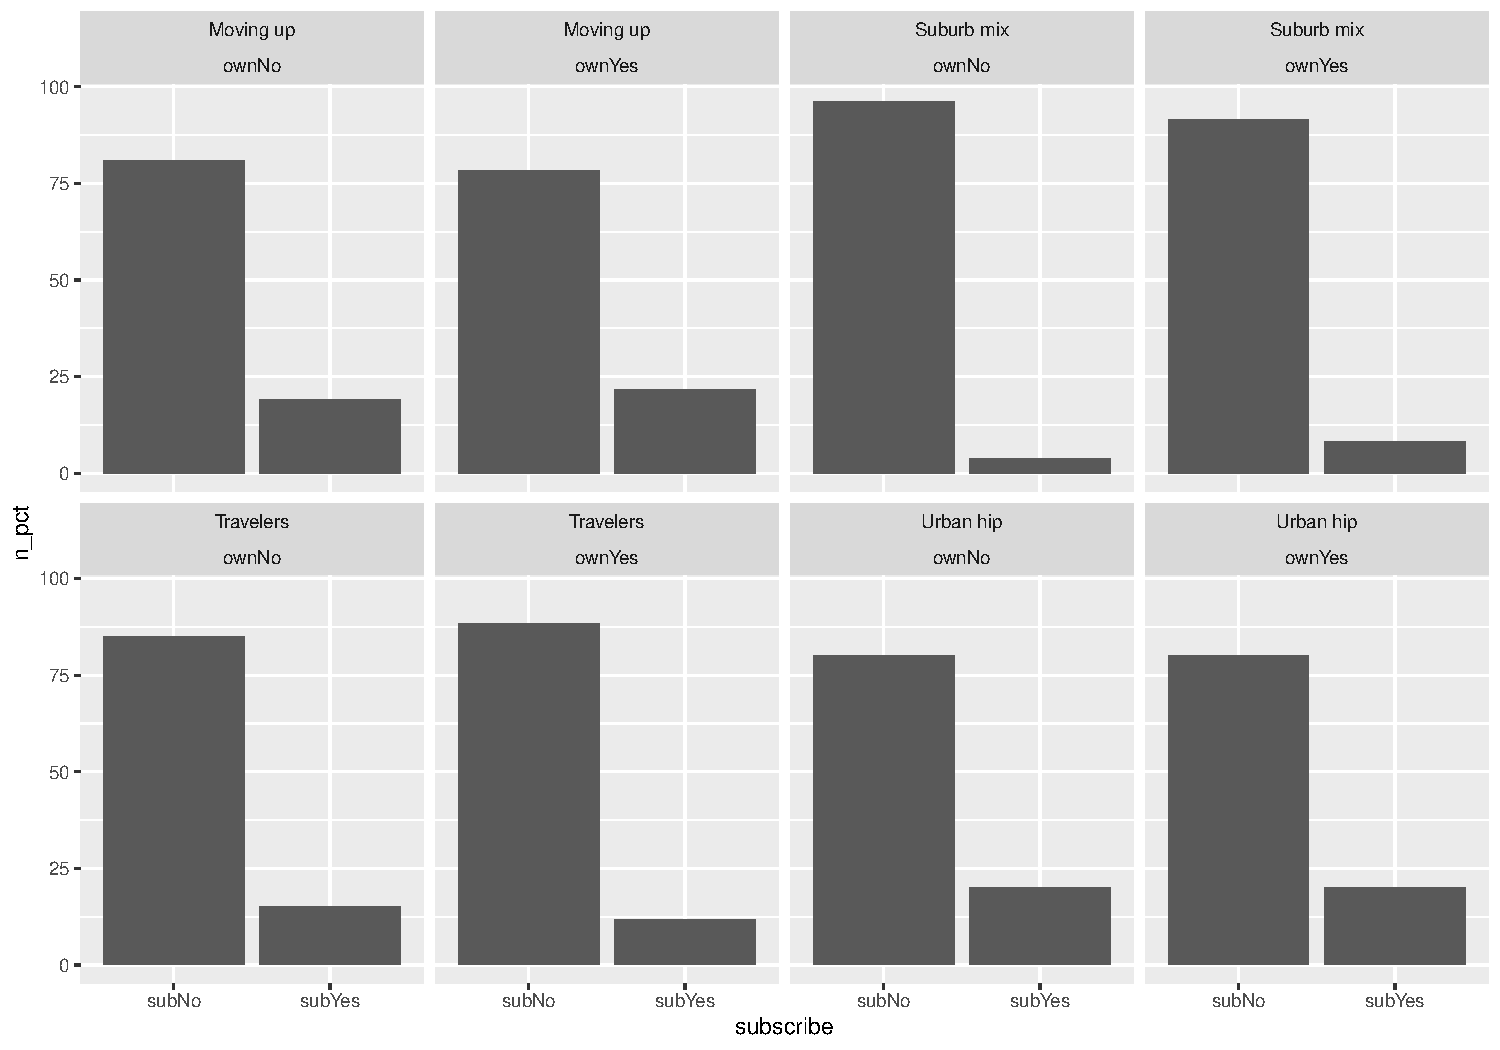
\includegraphics[width=0.5\textwidth,height=\textheight]{005_comparing_groups_tables_and_visualizations_files/figure-beamer/unnamed-chunk-12-1.pdf}
\end{center}
\end{frame}

\begin{frame}[fragile]{}
\phantomsection\label{section-15}
\begin{itemize}
\tightlist
\item
  \textbf{Visualization by group as proportions: the lattice way}
\end{itemize}

\tiny

\begin{Shaded}
\begin{Highlighting}[]
\CommentTok{\# Prepare data}
\NormalTok{prop\_table }\OtherTok{\textless{}{-}} \FunctionTok{table}\NormalTok{(segmentation}\SpecialCharTok{$}\NormalTok{subscribe,}
\NormalTok{                    segmentation}\SpecialCharTok{$}\NormalTok{Segment) }\SpecialCharTok{|\textgreater{}}
  \FunctionTok{prop.table}\NormalTok{(}\AttributeTok{margin =} \DecValTok{2}\NormalTok{) }\SpecialCharTok{|\textgreater{}}
\NormalTok{  \_[}\DecValTok{2}\NormalTok{, ] }\CommentTok{\# You can use \_ as a placeholder. Check ?pipeOp}
\end{Highlighting}
\end{Shaded}

\begin{Shaded}
\begin{Highlighting}[]
\FunctionTok{barchart}\NormalTok{(prop\_table, }
         \AttributeTok{xlab=}\StringTok{\textquotesingle{}Subscriber proportion by Segment\textquotesingle{}}\NormalTok{, }\AttributeTok{col=}\StringTok{\textquotesingle{}darkolivegreen\textquotesingle{}}\NormalTok{)}
\end{Highlighting}
\end{Shaded}

\begin{center}
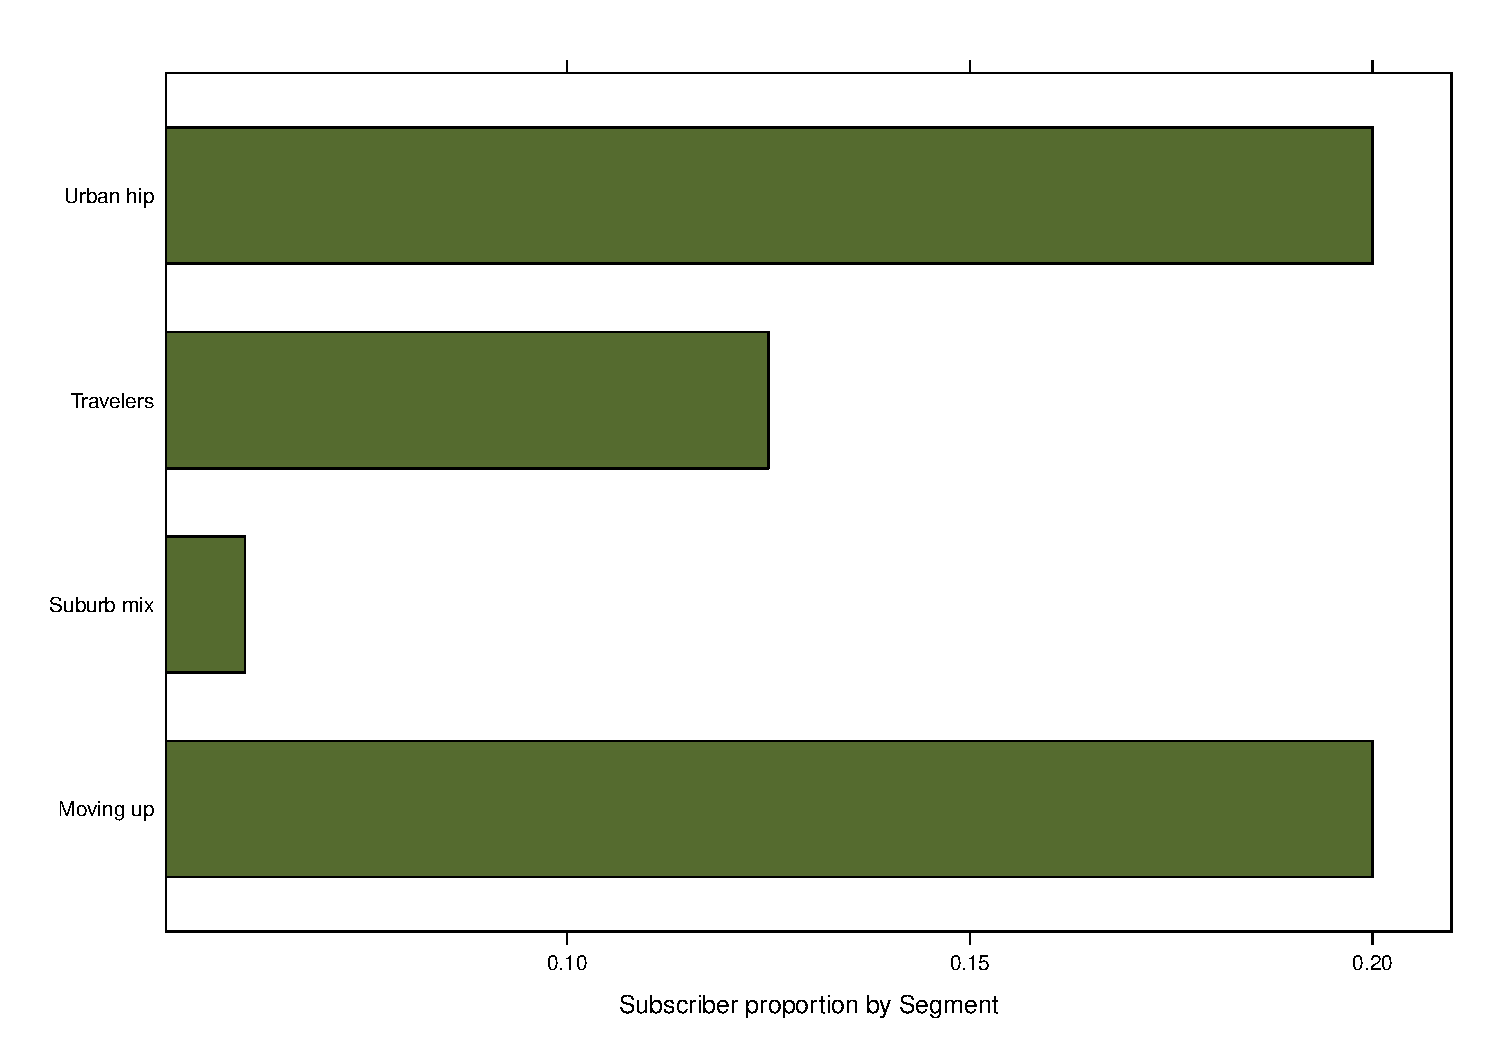
\includegraphics[width=0.5\textwidth,height=\textheight]{005_comparing_groups_tables_and_visualizations_files/figure-beamer/unnamed-chunk-14-1.pdf}
\end{center}
\end{frame}

\begin{frame}[fragile]{}
\phantomsection\label{section-16}
\begin{itemize}
\tightlist
\item
  \textbf{Visualization by group as proportions: the tidyverse way}
\end{itemize}

\tiny

\begin{Shaded}
\begin{Highlighting}[]
\CommentTok{\# Prepare data}
\NormalTok{prop\_table }\OtherTok{\textless{}{-}}\NormalTok{ segmentation }\SpecialCharTok{|\textgreater{}}
  \FunctionTok{count}\NormalTok{(subscribe, Segment) }\SpecialCharTok{|\textgreater{}}
  \FunctionTok{group\_by}\NormalTok{(Segment) }\SpecialCharTok{|\textgreater{}}
  \FunctionTok{mutate}\NormalTok{(}\AttributeTok{n\_pct =}\NormalTok{ n }\SpecialCharTok{/} \FunctionTok{sum}\NormalTok{(n)) }\SpecialCharTok{|\textgreater{}}
  \FunctionTok{filter}\NormalTok{(subscribe }\SpecialCharTok{==} \StringTok{\textquotesingle{}subYes\textquotesingle{}}\NormalTok{)}
\end{Highlighting}
\end{Shaded}

\begin{Shaded}
\begin{Highlighting}[]
\NormalTok{prop\_table }\SpecialCharTok{|\textgreater{}} \FunctionTok{ggplot}\NormalTok{() }\SpecialCharTok{+} 
  \FunctionTok{geom\_col}\NormalTok{(}\FunctionTok{aes}\NormalTok{(}\AttributeTok{x=}\NormalTok{n\_pct, }\AttributeTok{y=}\NormalTok{Segment),}
           \AttributeTok{fill=}\StringTok{\textquotesingle{}darkolivegreen\textquotesingle{}}\NormalTok{) }\SpecialCharTok{+}
  \FunctionTok{labs}\NormalTok{(}\AttributeTok{x=}\StringTok{\textquotesingle{}Subscriber proportion by Segment\textquotesingle{}}\NormalTok{, }
       \AttributeTok{y=}\ConstantTok{NULL}\NormalTok{)}
\end{Highlighting}
\end{Shaded}

\begin{center}
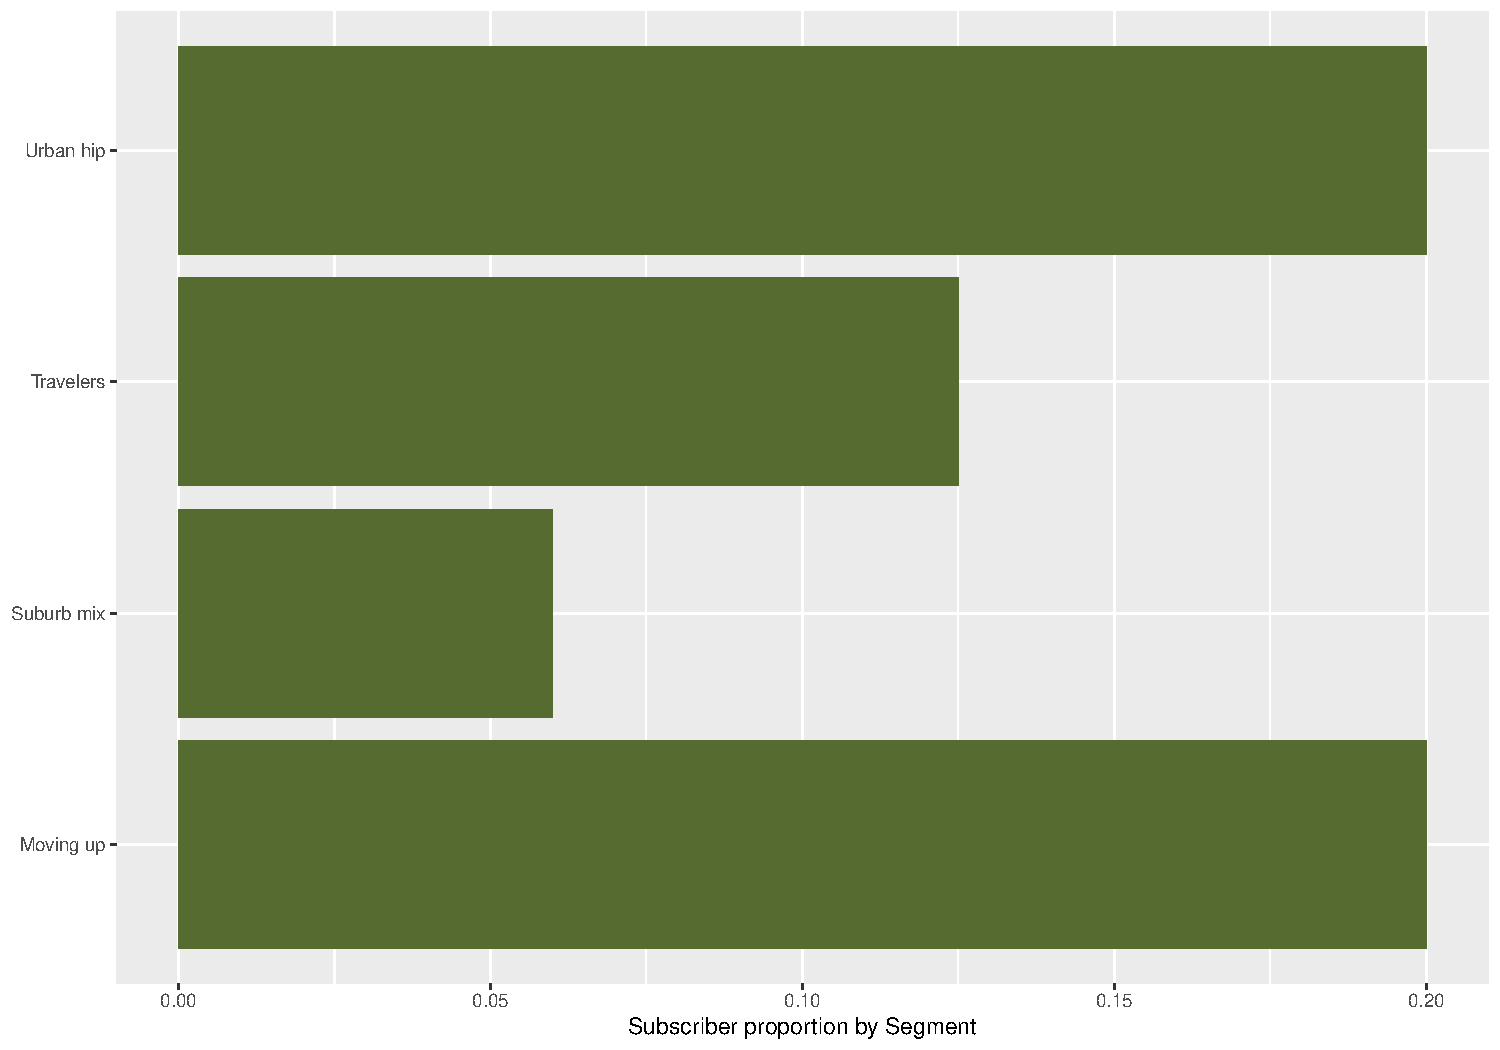
\includegraphics[width=0.5\textwidth,height=\textheight]{005_comparing_groups_tables_and_visualizations_files/figure-beamer/unnamed-chunk-16-1.pdf}
\end{center}
\end{frame}

\begin{frame}[fragile]{}
\phantomsection\label{section-17}
\begin{itemize}
\tightlist
\item
  \textbf{Visualization by group with continuous data: the lattice way}
\end{itemize}

\tiny

\begin{Shaded}
\begin{Highlighting}[]
\CommentTok{\# Prepare data}
\NormalTok{seg\_income\_agg }\OtherTok{\textless{}{-}} \FunctionTok{aggregate}\NormalTok{(income }\SpecialCharTok{\textasciitilde{}}\NormalTok{ Segment }\SpecialCharTok{+}\NormalTok{ ownHome, }
                            \AttributeTok{data=}\NormalTok{segmentation, }\AttributeTok{FUN =}\NormalTok{ mean)}
\end{Highlighting}
\end{Shaded}

\begin{Shaded}
\begin{Highlighting}[]
\FunctionTok{barchart}\NormalTok{(income }\SpecialCharTok{\textasciitilde{}}\NormalTok{ Segment, }\AttributeTok{data =}\NormalTok{ seg\_income\_agg,}
         \AttributeTok{groups=}\NormalTok{ownHome, }\AttributeTok{auto.key=}\ConstantTok{TRUE}\NormalTok{, }\CommentTok{\# Add groups}
         \AttributeTok{par.settings=}\FunctionTok{simpleTheme}\NormalTok{(}\AttributeTok{col=}\FunctionTok{terrain.colors}\NormalTok{(}\AttributeTok{n =} \DecValTok{2}\NormalTok{))) }\CommentTok{\# Change default colors}
\end{Highlighting}
\end{Shaded}

\begin{center}
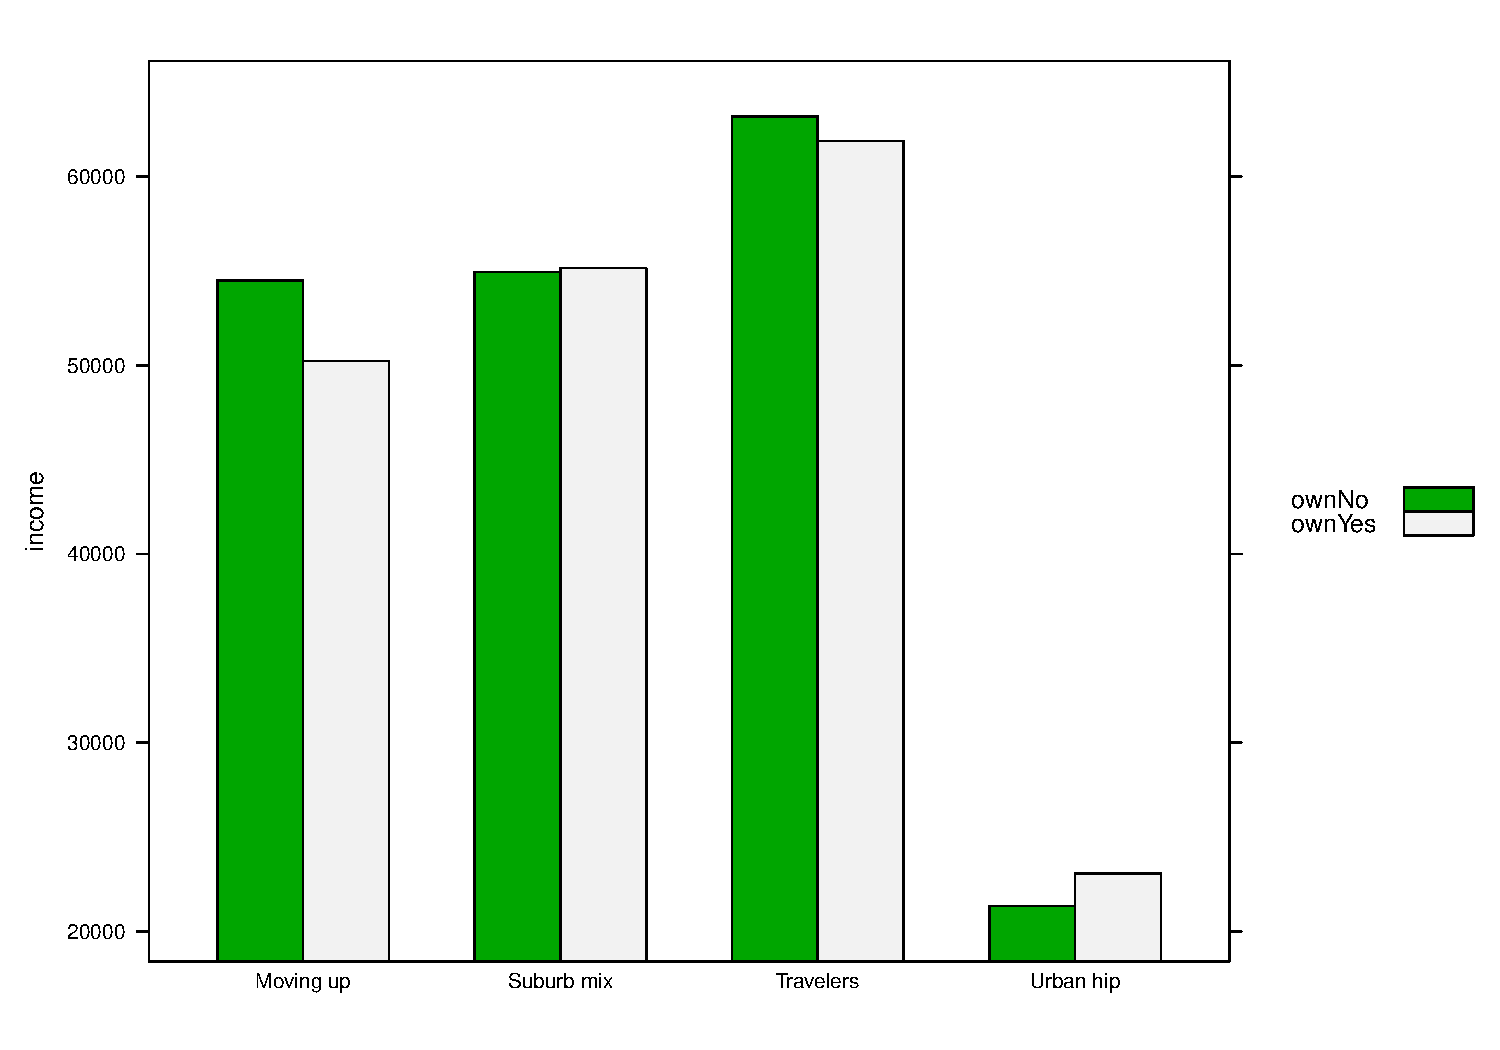
\includegraphics[width=0.5\textwidth,height=\textheight]{005_comparing_groups_tables_and_visualizations_files/figure-beamer/unnamed-chunk-18-1.pdf}
\end{center}
\end{frame}

\begin{frame}[fragile]{}
\phantomsection\label{section-18}
\begin{itemize}
\tightlist
\item
  \textbf{Visualization by group with continuous data: the tidyverse
  way}
\end{itemize}

\tiny

\begin{Shaded}
\begin{Highlighting}[]
\CommentTok{\# Prepare data}
\NormalTok{seg\_income\_agg }\OtherTok{\textless{}{-}}\NormalTok{ segmentation }\SpecialCharTok{|\textgreater{}} 
  \FunctionTok{group\_by}\NormalTok{(Segment, ownHome) }\SpecialCharTok{|\textgreater{}} 
  \FunctionTok{summarise}\NormalTok{(}\AttributeTok{mean\_income =} \FunctionTok{mean}\NormalTok{(income)) }\SpecialCharTok{|\textgreater{}} 
  \FunctionTok{ungroup}\NormalTok{()}
\end{Highlighting}
\end{Shaded}

\begin{Shaded}
\begin{Highlighting}[]
\NormalTok{seg\_income\_agg }\SpecialCharTok{|\textgreater{}} \FunctionTok{ggplot}\NormalTok{() }\SpecialCharTok{+}
  \FunctionTok{geom\_col}\NormalTok{(}\FunctionTok{aes}\NormalTok{(}\AttributeTok{x=}\NormalTok{Segment, }\AttributeTok{y=}\NormalTok{mean\_income, }\AttributeTok{fill=}\NormalTok{ownHome),}
           \AttributeTok{position =} \FunctionTok{position\_dodge}\NormalTok{(), }\AttributeTok{color=}\StringTok{\textquotesingle{}black\textquotesingle{}}\NormalTok{) }\SpecialCharTok{+}
  \FunctionTok{scale\_fill\_manual}\NormalTok{(}\AttributeTok{values=}\FunctionTok{terrain.colors}\NormalTok{(}\AttributeTok{n =} \DecValTok{2}\NormalTok{))}
\end{Highlighting}
\end{Shaded}

\begin{center}
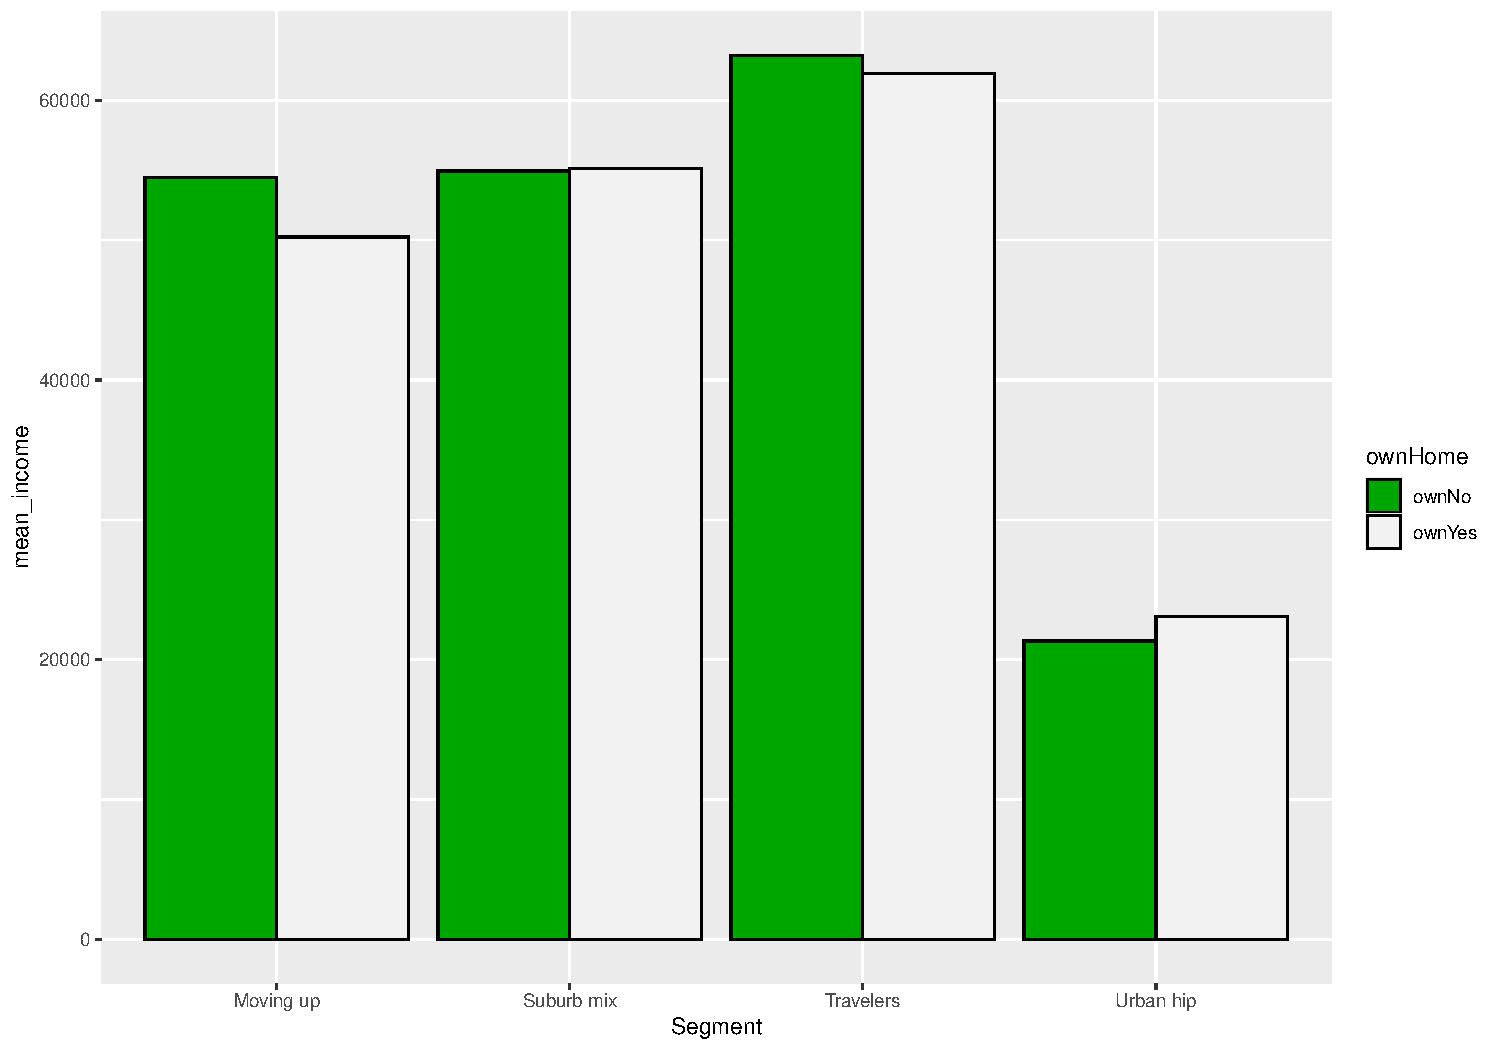
\includegraphics[width=0.5\textwidth,height=\textheight]{005_comparing_groups_tables_and_visualizations_files/figure-beamer/unnamed-chunk-20-1.pdf}
\end{center}
\end{frame}

\begin{frame}[fragile]{}
\phantomsection\label{section-19}
\begin{itemize}
\tightlist
\item
  \textbf{Visualization by group with continuous data: the lattice way}
\end{itemize}

\tiny

\begin{Shaded}
\begin{Highlighting}[]
\FunctionTok{bwplot}\NormalTok{(Segment }\SpecialCharTok{\textasciitilde{}}\NormalTok{ income }\SpecialCharTok{|}\NormalTok{ ownHome,}
       \AttributeTok{data =}\NormalTok{ segmentation,}
       \AttributeTok{xlab =} \StringTok{\textquotesingle{}Income\textquotesingle{}}\NormalTok{)}
\end{Highlighting}
\end{Shaded}

\begin{center}
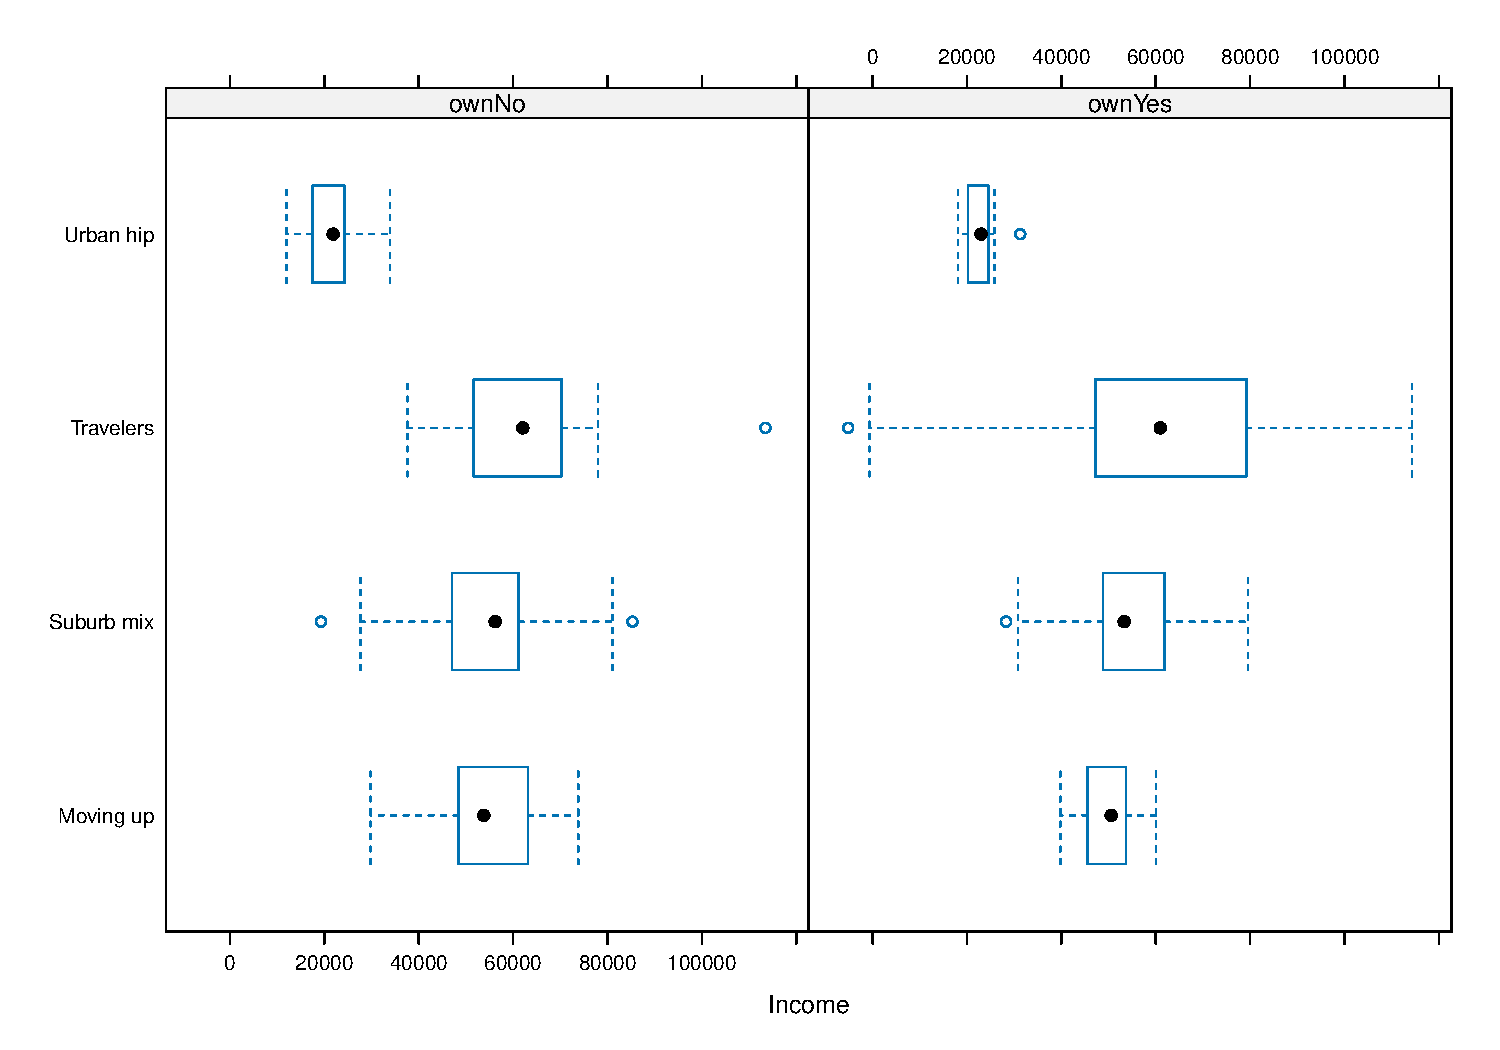
\includegraphics[width=0.5\textwidth,height=\textheight]{005_comparing_groups_tables_and_visualizations_files/figure-beamer/unnamed-chunk-21-1.pdf}
\end{center}
\end{frame}

\begin{frame}[fragile]{}
\phantomsection\label{section-20}
\begin{itemize}
\tightlist
\item
  \textbf{Visualization by group with continuous data: the lattice way}
\end{itemize}

\tiny

\begin{Shaded}
\begin{Highlighting}[]
\NormalTok{segmentation }\SpecialCharTok{|\textgreater{}} \FunctionTok{ggplot}\NormalTok{() }\SpecialCharTok{+}
  \FunctionTok{geom\_boxplot}\NormalTok{(}\FunctionTok{aes}\NormalTok{(}\AttributeTok{x=}\NormalTok{income, }\AttributeTok{y=}\NormalTok{Segment)) }\SpecialCharTok{+}
  \FunctionTok{facet\_wrap}\NormalTok{(}\AttributeTok{facets =} \FunctionTok{vars}\NormalTok{(ownHome)) }\SpecialCharTok{+}
  \FunctionTok{labs}\NormalTok{(}\AttributeTok{x=}\StringTok{\textquotesingle{}Income\textquotesingle{}}\NormalTok{,}
       \AttributeTok{y=}\ConstantTok{NULL}\NormalTok{)}
\end{Highlighting}
\end{Shaded}

\begin{center}
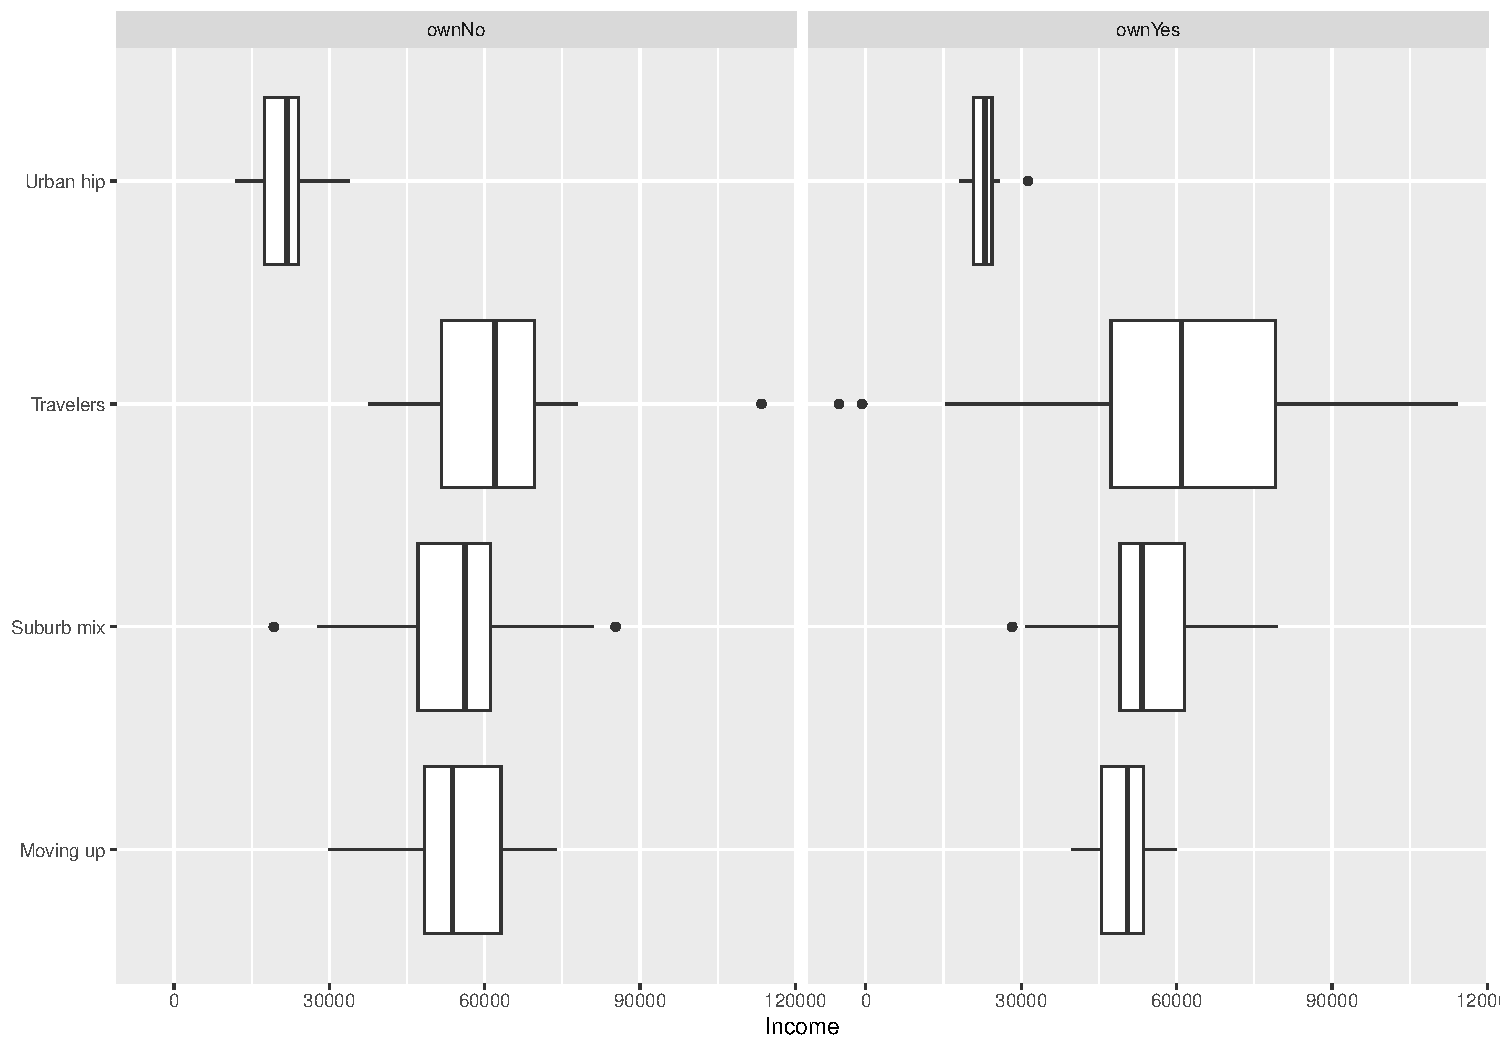
\includegraphics[width=0.5\textwidth,height=\textheight]{005_comparing_groups_tables_and_visualizations_files/figure-beamer/unnamed-chunk-22-1.pdf}
\end{center}
\end{frame}

\section{Acknowledgments}\label{acknowledgments}

\begin{frame}{}
\phantomsection\label{section-21}
\begin{itemize}
\item
  To my family that supports me
\item
  To the taxpayers of Colombia and the
  \href{https://www.umng.edu.co/estudiante}{\textbf{UMNG students}} who
  pay my salary
\item
  To the \href{https://www.business-science.io/}{\textbf{Business
  Science}} and \href{https://www.rfordatasci.com/}{\textbf{R4DS Online
  Learning}} communities where I learn
  \href{https://www.r-project.org/about.html}{\textbf{R}} and
  \href{https://www.python.org/about/}{\textbf{\(\pi\)-thon}}
\item
  To the \href{https://www.r-project.org/contributors.html}{\textbf{R
  Core Team}}, the creators of
  \href{https://posit.co/products/open-source/rstudio/}{\textbf{RStudio
  IDE}}, \href{https://quarto.org/}{\textbf{Quarto}} and the authors and
  maintainers of the packages
  \href{https://CRAN.R-project.org/package=tidyverse}{\textbf{tidyverse}}
  and
  \href{https://CRAN.R-project.org/package=tinytex}{\textbf{tinytex}}
  for allowing me to access these tools without paying for a license
\item
  To the \href{https://www.kernel.org/category/about.html}{\textbf{Linux
  kernel community}} for allowing me the possibility to use some
  \href{https://static.lwn.net/Distributions/}{\textbf{Linux
  distributions}} as my main
  \href{https://en.wikipedia.org/wiki/Operating_system}{\textbf{OS}}
  without paying for a license
\end{itemize}
\end{frame}

\section*{References}\label{references}
\addcontentsline{toc}{section}{References}

\begin{frame}[allowframebreaks]{References}
\phantomsection\label{refs}
\begin{CSLReferences}{1}{0}
\bibitem[\citeproctext]{ref-chapman_r_2019}
Chapman, Chris, and Elea McDonnell Feit. 2019. \emph{R {For} {Marketing}
{Research} and {Analytics}}. 2nd ed. 2019. Use {R}! Cham: Springer
International Publishing : Imprint: Springer.
\url{https://doi-org.ezproxy.umng.edu.co/10.1007/978-3-030-14316-9}.

\end{CSLReferences}
\end{frame}




\end{document}
